\section{Análisis bivariado}
\label{sec:analisis_bivariado}

\newcommand{\squarederr}[1]{
    \sum\limits_{t=1}^n \varnorm{#1}^2
}

\newcommand{\crosscorr}[2]{
  \frac{\sum\limits_{t=|k|+1}^n \varnorm{#1} (#2_{t-k} - \mu_{#2})}{
    \sqrt{\squarederr{#1} \squarederr{#2}}
  } \\
}

\newcommand{\corrdenom}{\sqrt{\squarederr{A}\squarederr{B}}}

En \cite{KOU2008.2} se continúa el trabajo en series de tiempo, y se efectúan análisis tanto para cada serie por separado como para las dos en conjunto, lo cual se llama ``análisis bivariado'' en la terminología de series de tiempo. En este análisis pretendemos analizar ambas series como parte de un sistema y ver cómo se influyen y retroalimentan mutuamente.

Una posible medida del \entrainment se podría obtener midiendo cuánto influye una serie sobre otra, considerándolas a ambas como parte de un sistema donde ambas interactúan. Este \entrainment, entonces, sería direccional: queremos medir cuánto influye el interlocutor $A$ sobre el interlocutor $B$ y viceversa. Puede darse el caso en que ambos tengan fuerte interacción, en tal caso hablamos de \emph{feedback}.

Para medir cuánto se mimetizan las dos series, utilizaremos la función de correlación cruzada (f.c.c) \cite{CHATFIELD}, que mide cuánto se parecen la serie $X$ e $Y$ aplicando un desplazamiento $k$, lo cual nos arroja como resultado un valor entre $-1$ y $1$ (similar al coeficiente de correlación de la estadística clásica). Podemos aproximar la c.c.f. mediante la fórmula de la correlación cruzada muestral.

\begin{equation}
  \label{cross_correlation_definition}
  r_{AB}(k) =
  \left\{
    \begin{array}{ll}
      \frac{\sum\limits_{t=k+1}^n \varnorm{A} (B_{t-k} - \mu_{B})}{\corrdenom} \\ & \mbox{si } k \geq 0 \\
      \frac{\sum\limits_{t=-k+1}^n \varnorm{B} (A_{t+k} - \mu_{A})}{\corrdenom} \\  & \mbox{si } k < 0
    \end{array}
  \right.
\end{equation}

Podemos ver que, si $k \geq 0$, lo que hacemos es, a grandes rasgos, calcular la correlación de Pearson entre $A$ y $B$, pero tomando los $n-k$ últimos valores de $A$ y los $n-k$ primeros de $B$. Si $k < 0$, lo hacemos entre $A$ y $B$, pero desplazando en sentidos inversos. Viéndolo de otra forma, si $k \geq 0$, estamos midiendo cuánto influye $B$ sobre $A$ contemplando un desplazamiento de $k$ puntos; si $k \leq 0$ medimos la influencia de $A$ sobre $B$ a misma distancia. La utilización de estos desplazamientos está explicada en \cite{gravano2015backward}, donde se menciona que la influencia de los hablantes no es necesariamente inmediata sino que puede tener algunos segundos de demora para tomar lugar.


Para cada conversación, se estima entonces el correlograma cruzado, considerando desplazamientos tanto positivos como negativos. Hecho esto, en el estudio \cite{KOU2008.2} sólo analizan la significancia de los resultados de la correlación cruzada, enumerando aquellos lags en los cuales esto ocurrió. En la sección \ref{sec:method_entrainment} comentaremos cómo utilizamos la técnica descripta para la medición del entrainment direccional.

\begin{figure}
\centering
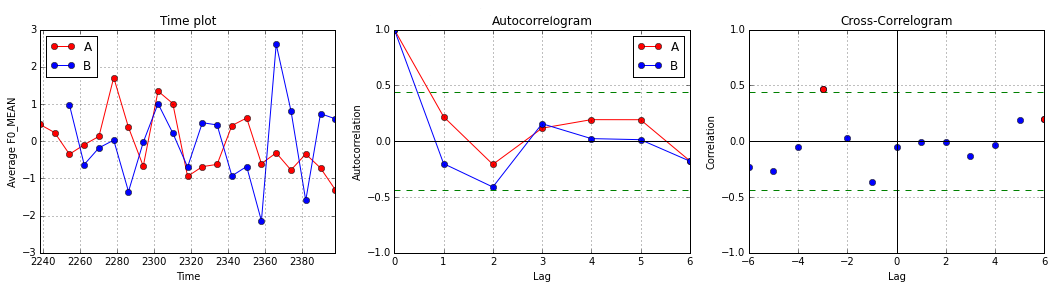
\includegraphics[width=\textwidth]{images/time_plot_with_cross_correlation.png}
\caption{Time-plot producido por TAMA, junto a su autocorrelación y correlación cruzada}
\end{figure}
